\section{Cos’è un cifrario a sostituzione? E a trasposizione?}

Le reti inizialmente venivano utilizzate da ricercatori universitari per scambiarsi e-mail, e dalle aziende per condividere le stampanti, di conseguenza la sicurezza aveva un ruolo marginale.

Oggi le reti sono utilizzate da milioni di persone per fare acquisti, lavorare con la banca o per documenti importanti. Questo fa diventare la sicurezza qualcosa di fondamentale e ricercato in quanto sempre più persone malintenzionate cercano di rubare dati sensibili.
La crittografia serve a rendere un messaggio non comprensibile/leggibile a persone non autorizzate a leggerlo.
\subsection{Cos'è il cifrario a sostituzione}
Per cifrare un messaggio ci sono diverse tecniche, una di queste è il \textbf{cifrario a sostituzione} (per cifrario s’intende una trasformazione carattere per carattere, senza considerare la struttura linguistica del messaggio). Uno dei cifrari più antichi che si conoscono è il cifrario di Cesare.
\subsection{Cos'è il cifrario a trasposizione}
Il sistema generale sta nel sostituire appunto un carattere/coppie di lettere/sillabe/ecc con altre.
Un altro tipo di cifrario è il \textbf{cifrario a trasposizione} che riordina le lettere senza mascherarle come fa il cifrario a sostituzione.

Un esempio è la trasposizione colonnare che funziona come segue: tramite una parola chiave si numerano le colonne, il testo in chiaro va disposto di seguito sulle colonne. Successivamente si ordinano le colonne in base alla parola chiave, ad ogni lettera viene dato un valore dipendente dal valore della lettera nell’alfabeto, successivamente si riscrive per colonne il testo cifrato.

\subsection{Differenze tra i due}
Le differenze sostanziali tra i due è che nel cifrario a sostituzione l’ordine rimane invariato ma le lettere vengono mascherate, in quello a trasposizione le lettere non vengono mascherate e il testo viene mescolato (secondo opportuni criteri).

\section{Si descriva il block cipher}
\subsection{Cos'è}
Block cipher è un algoritmo a chiave simmetrica (tecnica di cifratura in cui la chiave è la stessa sia per la crittazione sia per la decrittazione) operante su un gruppo di bit di lunghezza finita organizzati in un blocco.
Questo tipo di algoritmi sono composti da due parti, una che cifra (E) e un’altra che decifra ($E_1$).
Dati n bit in entrata in blocco, l’algoritmo cifra n bit in blocco.
Per eseguire la crittazione e la decrittazione è possibile implementarli tramite semplici circuiti elettrici, come ad esempio la P-box (scatola di permutazione) o la S-box (scatole di sostituzione).
\subsection{P-box}
La P-box permette di trasporre 8 bit, se un input è lineare 01234567, l’output è 24506713, ovviamente la P-box lavora alla velocità della luce, in quanto non sono necessari calcoli, però è necessario conoscere la chiave di cifratura (ossia come sono disposti i collegamenti interni della P-box).
\subsection{S-box}
la S-box invece è un altro tipo di circuito che sostituisce il numero di bit del messaggio, mescolandoli.
Se il messaggio in entrata ha m bit, l’output è da n. Ad esempio si ha un input di 8 bit, l’output sarà da 3 bit permutati dagli 8, servirà poi una S-box per decifrare il messaggio e tornare agli 8 bit originali. 


\begin{figure}[H]
\centering
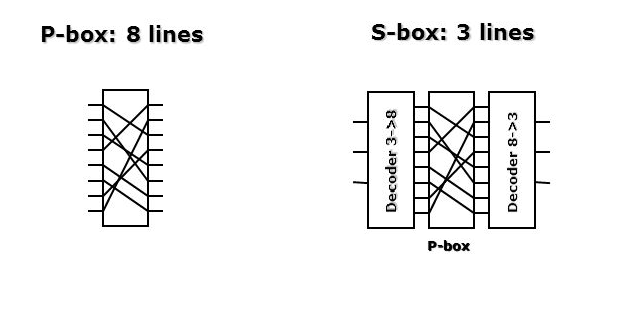
\includegraphics[scale=0.6]{res/img/52_P-boxS-box.png}
%\caption{Didascalia dellimmagine}
\end{figure}

\subsection{Pregi}
Combinati insieme, P-box e S-box, creano un sistema crittografico molto performante.
\subsection{Difetti}
Singolarmente questi metodi non sono molto affidabili, S-box è molto vulnerabile agli attacchi basati sul tempo.
\subsection{Ambiti d'uso}
Utilizzati in crittografia per cifrare blocchi di dati (a differenza degli algoritmi di flusso che cifrano un solo elemento alla volta).

\section{Si descriva l’algoritmo DES e triplo DES}
\subsection{Cos'è DES?}
DES (Data Encryption Standard) è un algoritmo di cifratura scelto come standard, prima dal governo degli Stati Uniti e successivamente è diventato di utilizzo internazionale.

Si basa su un algoritmo a chiave simmetrica (Usa la stessa chiave per la crittografia e per la decrittazione) con chiave a 64bit (solo 56 utili, gli altri 8 sono di controllo).
DES è un perfetto esempio di cifrario a blocchi, è un algoritmo che prende in ingresso una stringa di lunghezza fissa di testo in chiaro e, con una serie di operazioni complesse, da in output una stringa di testo della stessa lunghezza.

DES è formato da 19 stadi distinti:
\begin{itemize}
\item	il primo traspone semplicemente i 64 bit di testo in chiaro, l’ultimo fa il contrario.
\item	Il penultimo stadio scambia i 32 bit più a sinistra con i 32 più a destra.
\item	Gli altri 16 stadi sono funzionalmente identici, ma sono parametrizzati da funzioni diverse della chiave.
\end{itemize}

\subsection{Cos'è Triplo-DES?}
Per migliorare la complessità dell’algoritmo viene implementato un nuovo metodo chiamato triplo DES. Nel triplo DES vengono utilizzate due chiavi e tre stadi. Nel primo stadio il testo viene cifrato con il sopracitato DES usando la chiave $K_1$, nel secondo stadio DES viene usato in modalità di decifrazione usando la chiave $K_2$. Infine, un’ultima cifratura viene fatta con $K_1$. È un metodo Encrypt Decrypt Encrypt (EDE). Il metodo EDE è stato scelto in quanto risulta compatibile con i computer che usano la cifratura singola, semplicemente impostando $K_1=K_2$.

AES (Advanced Encryption Standard) sostituisce triplo DES (quindi anche DES).

\begin{figure}[H]
\centering
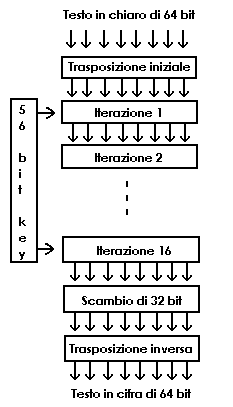
\includegraphics[scale=0.8]{res/img/53_DES.png}
%\caption{Didascalia dellimmagine}
\end{figure}

\subsection{Pregi}
Permettono una cifratura a blocchi rispetto al singolo elemento come la cifratura a flusso.\\
Triplo DES migliora la poca sicurezza del DES.\\
Triplo DES è compatibile con DES grazie alla sua composizione, basta porre $K_1=K_2$.

\subsection{Difetti}
A causa della dimensione ridotta della chiave (64 bit) DES non è molto sicuro.\\
Usando questi metodi crittografici un testo in chiaro produrrà sempre il medesimo testo cifrato.\\
Entrambi soffrono di una prestazione software.\\
Entrambi gli algoritmi sono stati sostituiti da AES.

\subsection{Ambiti d'uso}
Nell'ambito della crittografia, stanno cadendo in disuso a causa delle scarse prestazioni, sostituiti da AES.

\section{Counter Mode Cipher}
\subsection{Causa della creazione}
La maggior parte delle tecniche di cifratura hanno il problema di rendere impossibile l’accesso casuale ai dati. Questo è un problema quando ad esempio si va accede ad un file su disco in ordine non sequenziale (random), se il file è cifrato con il cipher block chaining (tecnica che cifra i blocchi basandosi sui blocchi precedenti) allora bisogna prima decifrare tutti i blocchi precedenti, questo può diventare inutilmente oneroso.
\subsection{Cos'è?}
Per questo motivo è stata creata la modalità contatore. In questo caso il testo in chiaro non viene cifrato direttamente; si cifra invece un vettore d’inizializzazione (IV) con una costante (K), successivamente il risultato viene messo in XOR con il testo in chiaro. Si incrementa di 1 il vettore d’inizializzazione ad ogni blocco, diventa facile riuscire a decifrare un blocco in qualunque posizione esso si trovi, senza decifrare prima i suoi predecessori.

\begin{figure}[H]
\centering
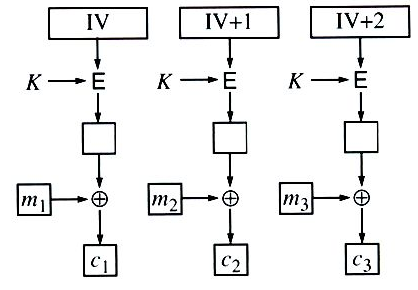
\includegraphics[scale=0.6]{res/img/54_CMC.png}
%\caption{Didascalia dellimmagine}
\end{figure}

\subsection{Pregi}
Permette la decifratura di blocchi di dati in ordine non sequenziale, non necessita quindi di decrittare tutti i blocchi a lui precedenti.

\subsection{Difetti}
Se si utilizza la stessa chiave e lo stesso IV per due differenti messaggi, avendo i due messaggi cifrati è possibile bypassare la sicurezza facendo lo XOR dei due messaggi, ottenendo la chiave.

\subsection{Ambiti d'uso}
Viene utilizzato nella cifratura come alternativa agli algoritmi che cifrano i dati basandosi su blocchi precedenti.\\
Utile ad esempio se si necessita di effettuare ricerche non sequenziali dei dati.

\section{Cipher block chaining}

DES, triplo DES e AES, utilizzano un cifrario a sostituzione monoalfabetica che usa caratteri lunghi. Usando sempre la stessa chiave, ottenendo sempre blocchi di testo cifrato uguali (per testo in chiaro uguale), risulta semplice (con un po’ di forza bruta) compromettere la sicurezza dei blocchi cifrati con queste tecniche.
\subsection{Cos'è?}
Un modo per evitare questo problema è collegare tutti i blocchi cifrati in modo diverso, questa tecnica è chiamata Cipher block chaining.
In questo metodo, ogni blocco di testo in chiaro è messo in XOR con il precedente blocco cifrato prima di eseguire la cifratura vera e propria.

Così facendo a blocchi di testo in chiaro uguali non corrispondono più blocchi di testo cifrato identici. Per il primo blocco di questa catena lo XOR viene calcolato con un blocco di dati casuali (vettore di inizializzazione IV), che è trasmesso (in chiaro) insieme al testo cifrato.

Questo metodo rende la criptoanalisi più difficile, con un grande incremento di sicurezza. Un problema è il fatto di rendere impossibile la decrittazione di un blocco in maniera casuale senza prima aver decrittato tutti i blocchi precedenti. Problema risolto dal counter mode cipher.

\begin{figure}[H]
\centering
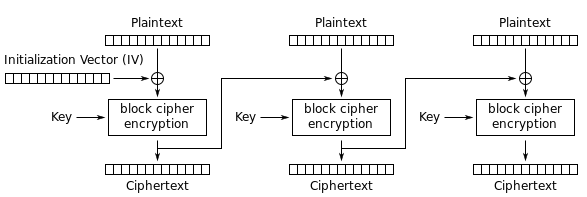
\includegraphics[scale=0.7]{res/img/55_CBC.png}
%\caption{Didascalia dellimmagine}
\end{figure}

\subsection{Pregi}
Migliora il problema dei cifrari che utilizzano sempre la stessa chiave (DES/TRIPLODES/AES), ovvero il problema di generare sempre blocchi uguali per testi uguali. 
\subsection{Difetti}
Per decifrare un blocco in mezzo al flusso bisogna prima decrittare tutti i blocchi a lui antecedenti.
\subsection{Ambiti d'uso}
Nell'ambito della cifratura, viene utilizzato quando è necessario un livello di sicurezza maggiore rispetto a AES, in quanto produce testo cifrato diverso per blocchi di testo in chiaro uguali.

\section{Stream cipher}
\subsection{Cos'è?}
Una variante dei cifrari a blocchi è stream cipher (cifrario di flusso).
Questa tecnica sfrutta un vettore di inizializzazione (IV) e una chiave, cifrate insieme generano un keystream che è indipendente dal testo in chiaro, successivamente si può cifrare nuovamente il keystream con la chiave, un numero arbitrario di volte per ottenere keystream differenti, con la quale poi verrà cifrato il testo in XOR.
Per la decrittazione viene eseguita generando lo stesso keystream dal lato del ricevente.

Questa tecnica permette un’alta elasticità agli errori, in quanto la keystream non dipende dai dati e su di essa si basa la cifratura di ogni blocco, di conseguenza un errore nel testo in chiaro vale come un errore nel testo cifrato (problema che riguardava il cipher block chaining).

Tuttavia, per utilizzare al meglio questa tecnica, IV e chiave non devono mai essere riutilizzati, altrimenti si genererebbe più volte lo stesso keystream, stessa cosa vale per la cifratura, non va mai utilizzato lo stesso keystream per cifrare un testo, altrimenti si viene esposti al problema del tipo keystream riutilizzato.

\begin{figure}[H]
\centering
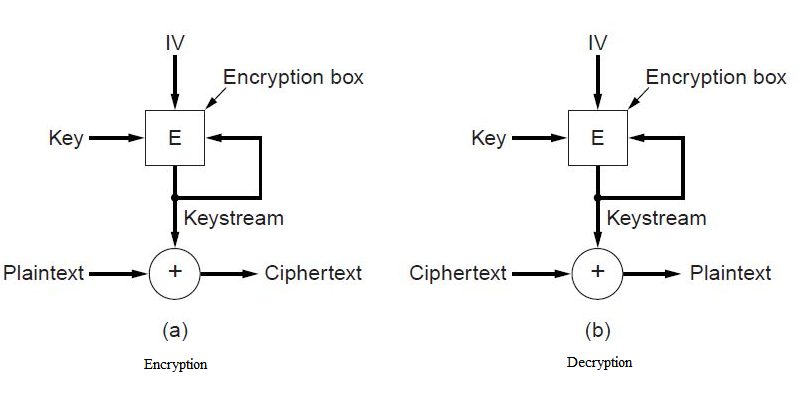
\includegraphics[scale=0.6]{res/img/56_StreamCipher.png}
%\caption{Didascalia dellimmagine}
\end{figure} 

\subsection{Pregi}
Garantisce alta elasticità agli errori.
\subsection{Difetti}
Ha il rischio di keystream riutilizzato se non si sta attenti.
\subsection{Ambiti d'uso}
Utilizzato per cifrare dati in applicazioni in cui è necessario che un bit di errore non rovini 64 bit di testo in chiaro.

\section{RSA}
\subsection{Causa della creazione}
Un grosso problema del sistema crittografico è sempre stata la distribuzione delle chiavi. 
È sempre stato assunto che le chiavi di cifratura e decifrazione fossero le stesse (o derivabili l’una dall’altra), e la chiave doveva essere distribuita a tutti gli utenti del sistema. Qualora un intruso riusciva a rubare una chiave, tutto il sistema andava a rotoli.

Una variante per le chiavi simmetriche (stessa chiave per decifrare e cifrare) è stato dato dalle chiavi asimmetriche (o chiavi pubbliche/private).
Questo sistema richiede che ogni utente sia in possesso di due chiavi, una pubblica per la cifratura e una privata per la decifratura, quella pubblica può essere condivisa al mondo, mentre quella privata dev’essere in possesso solo del proprietario.
Cosi facendo chiunque può scrivere un messaggio cifrato a chi vuole, basta cifrarlo con la chiave pubblica della persona interessata, la persona interessata poi usera la sua chiave privata per decifrarlo.
\subsection{Cos'è?}
RSA è un algoritmo di crittografia che cerca di trovare un modo per generare queste chiavi, in modo da renderle impossibili da dedurre tramite calcoli.
È considerato un algoritmo molto robusto, il suo maggior svantaggio è che richiede chiavi di almeno 1024 bit per poter offrire una buona sicurezza (contro i 128 bit degli algoritmi a chiave simmetrica) il che lo rende abbastanza lento.
Si basa su alcuni principi di teoria dei numeri che si possono riassumere in quattro punti:
\begin{itemize}
\item	Si scelgono due numeri primi, p e q (tipicamente di 1024 bit)
\item	Si calcola n=p*q    e   z=(p-1)*(q-1).
\item	Si sceglie un numero primo relativamente a z, detto d.
\item	Si trova e tale che e*d=1 mod z.
\end{itemize}

Si divide il testo in chiaro, P, in modo che 0$\leq$P<n. Per cifrare il messaggio P, calcoliamo C=$P^e$ (mod n). Per decifrare C calcoliamo P=$C^d$. Questo si può fare perché le funzioni di cifratura e decifrazione sono una l’inverso dell’altra.
La chiave pubblica quindi consiste nella coppia (e,n) mentre quella privata consiste in (d, n).

La sicurezza del metodo è basata sulla difficoltà di scomporre in fattori i numeri molto grandi.

\subsection{Pregi}
Algoritmo molto robusto, che permette lo scambio di chiavi con una sicurezza quasi assoluta.
\subsection{Difetti}
Richiede chiavi di almeno 1024 bit, il che rende l'algoritmo molto lento.
\subsection{Ambiti d'uso}
Viene utilizzato per lo scambio dati con persone sconosciute.

\section{Si descriva la tecnica di attacco “Birthday attack”}
\subsection{Firme digitali}
L’autenticità di molti documenti legali, finanziari ecc. è basata sulla presenza o assenza di una firma autografa autorizzata. Per questo esistono le firme digitali. Grazie a queste si può verificare l’autenticità di un documento. Queste firme si basano su protocolli crittografici comunemente utilizzati.

Per generare una firma digitale vengono utilizzate delle funzioni di hash, tra queste la funzione MD (message digest) che ha 4 importanti proprietà:
\begin{itemize}
\item	È facile calcolare MD(P) (P messaggio).
\item	Da MD(P) è praticamente impossibile trovare P.
\item	Dato P, nessuno è in grado di trovare P’ tale che MD(P’)=MD(P). (non è possibile trovare un testo la cui cifratura è uguale alla cifratura di un altro testo.
\item	Se l’input cambia anche solo di 1 bit, l’output diventa completamente diverso.
\end{itemize}
Grazie a queste proprietà la firma diventa estremamente sicura e può far da garante per documenti importanti.
\subsection{Cos'è il birthday attack}
Il birthday attack è un esempio per dimostrare che, per forzare una MD di m bit, bastano solamente $2^{m/2}$ operazioni. L’idea per quest’attacco viene da una tecnica che i professori di matematica usano spesso nei corsi di matematica: “Quanti studenti ci devono essere in una classe perché la probabilità che due persone abbiano lo stesso compleanno superi il 50\%?” (23).
Con 23 persone possiamo formare (23*22)/2=253 coppie differenti, ognuna ha probabilità 1/365 di essere quella buona, di conseguenza la percentuale di possibilità supera facilmente il 50\%.

Generalizzando questa idea: Se c’è una funzione fra input e output con n valori di input e k possibili valori di output, ci sono n(n-1)/2 coppie di input. Se n(n-1)/2>k la possibilità di avere una coppia con lo stesso output è decisamente alta: Per avere due output uguali basta avere n>$\sqrt{k}$.
Tutto questo significa che un MD di 64 bit, può essere forzato, con buona probabilità, generando 232 messaggi e cercandone due con lo stesso MD.

\section{Sicurezza in 802.11}
\subsection{Cos'è?}
Lo standard 802.11 (standard di trasmissione per le reti WLAN (Wireless LAN)) prescrive un protocollo per lo strato data link, questo protocollo è chiamato WEP (Wired Equivalent Privacy) il cui scopo è portare sulla LAN wireless la stessa sicurezza di quella cablata.
\subsection{Come funziona}
WEP utilizza uno stream cipher (cifratura di flusso a chiave simmetrica) basato sull’algoritmo RC4 per cifrare i dati e CRC-32 (controllo a ridondanza ciclica) per verificare l’integrità.
Nel WEP, RC4 è utilizzato per generare un keystream che viene applicato in XOR al testo in chiaro per produrre il testo cifrato. La keystream è generata partendo da un vettore di inizializzazione (IV), vettore che deve essere cambiato ad ogni invio per mantenere alta la sicurezza.
Il suo funzionamento è il seguente:
\begin{itemize}
\item	Viene calcolato il checksum del payload utilizzando il CRC-32.
\item	Il checksum viene aggiunto al payload per formare il testo in chiaro.
\item	Al testo in chiaro (payload+checksum) viene applicato in XOR una parte del keystream pari alla sua lunghezza. Il risultato è il testo cifrato.
\item	L’IV utilizzato per inizializzare il keystream RC4 viene inviato insieme al testo cifrato.
Quando il destinatario riceve il pacchetto:
\item	Estrae il payload cifrato.
\item	Genera il keystream a partire dalla chiave segreta condivisa e l’IV ricevuto.
\item	Calcola lo XOR fra il testo cifrato e il keystream ottenendo il testo in chiaro
\item	Verifica il checksum per vedere se ci sono state manomissioni.
\end{itemize}
Purtroppo, questo sistema non è molto affidabile, in quanto l’IV facilmente si ripete, generando il pericolo del riutilizzo del keystream e rendendo tutte le transazioni a rischio di letture indesiderate. WEP è stato già sostituito da nuovi sistemi più sicuri.

\subsection{Pregi}
Provvede una sicurezza basilare
\subsection{Difetti}
Non è per nulla affidabile visto che l'IV si ripete generando il pericolo di riutilizzo del keystream.
\subsection{Ambiti d'uso}
Ormai obsoleto, viene sostituito da sistemi più sicuri.

\section{Si descriva la sicurezza di Bluetooth}

Rispetto a 802.11, Bluetooth ha un raggio d’azione considerevolmente minore, tuttavia necessita di un buon grado di sicurezza.
La sicurezza in Bluetooth è divisa in 3 modalità diverse, che vanno da nessuna sicurezza a una completa sicurezza dei dati e controllo dell’integrità.
Generalmente la sicurezza bluetooth è tenuta disabilitata.
\subsection{Livelli di sicurezza}
La sicurezza Bluetooth inizia quando un nuovo dispositivo slave chiede un canale al master.
Questo controllo viene effettuato tramite passkey, generalmente salvate in entrambi i dispositivi e scambiate al momento del collegamento. Altre volte è una chiave interna ad un dispositivo che va poi inserita all’interno di un altro sotto forma di numero decimale.
Quando si stabilisce un canale, master e slave controllano se l’altro conosce la passkey, in caso affermativo negoziano se il canale dev’essere cifrato e/o se bisogna effettuare il controllo di integrità.
La cifratura usa uno stream cipher (cifratura a flusso a chiave simmetrica) e per il controllo d’integrità usa Safer+ (altro cifrario a blocco con chiave simmetrica).

Un altro problema di bluetooth è che autentica solo i dispositivi, e non gli utenti, quindi il furto di un dispositivo bluetooth lascia l’accesso a tutti i dati del proprietario precedente.
Bluetooth implementa però la sicurezza anche in strati superiori al data link, tipo con password o PIN per completare la transazione.

\subsection{Pregi}
Diverse modalità di sicurezza, sicurezza implementata in diversi strati per mantenerla alta.
\subsection{Difetti}
Questo sistema di sicurezza purtroppo non protegge nel caso di furto del dispostivo.
\subsection{Ambiti d'uso}
Utilizzato nelle connessioni bluetooth.

\section{La tecnica di attacco reflection attack}
\subsection{Cos'è?}
Il reflection attack è una tipologia di attacco informatico che sfrutta delle falle nei protocolli di autenticazione (servono per autenticare l’identità in caso di scambio di messaggi) cercando di simulare diverse entità.

In questa tipologia di attacco sono necessari due interlocutori, A e B, e dev’essere aprire più conversazioni contemporaneamente con la vittima (B).
C , il nostro malintenzionato, seguendo alcune procedure e scambi multipli riesce a simulare l’identità di A, imbrogliando B, e potenzialmente aver accesso a tutte le conoscenze private di A che conosce B. (immaginando che B sia una banca, C che finge di essere A, ha libero accesso ai suoi soldi, non è proprio una cosa carina).
\subsection{Regole per evitarlo}
Questo attacco porta a generare 4 regole per la buona riuscita di un protocollo di autenticazione:
\begin{itemize}
\item	Fare in modo che chi inizia l’autenticazione provi la sua identità prima che lo faccia chi risponde.
\item	Far si che entrambi gli interlocutori utilizzino chiavi differenti per provare la propria identità.
\item	Far si che gli interlocutori usino (per le richieste) numeri presi da insiemi diversi.
\item	Rendere il protocollo resistente a attacchi che coinvolgono una seconda sessione parallela.
\end{itemize}
Se anche una sola di queste regole viene meno, il protocollo può essere forzato.

\section{Replay attack}
\subsection{Cos'è?}
Il replay attack è una tipologia di attacco informatico che sfrutta le falle nei protocolli di autenticazione (servono per autenticare l’identità in caso di scambio di messaggi), cercando di simulare diverse identità e potenzialmente rubare dati.

Simile all’attacco Man-in-the-middle il replay attack consiste nell'impossessarsi di una credenziale di autenticazione comunicata da un host ad un altro, e riproporla successivamente simulando l'identità dell'emittente. La differenza con il Man-in-the-middle sta nell’asincronia dell’operazione: mentre in MITM le operazioni avvengono in tempo reale, nel replay attack l’azione fraudolenta può essere eseguita anche a distanza di giorni.

Un esempio si ha quando A invia una richiesta di bonifico alla propria banca (B), C intercetta i messaggi e li salva. Dopo un certo tempo C rispedisce gli stessi messaggi a B. B, credendo di parlare con A, esegue le istruzioni. 
\subsection{Metodi per evitarlo}
Esistono diversi metodi per impedire questo tipo di attacchi, uno è inserire un timestamp ai messaggi, cosi da evitare una ritrasmissione futura (vulnerabile, in quanto qualsiasi finestra temporale si metta per la validità dei messaggi, C può sempre sfruttarla).
Un secondo metodo è inserire dei nonce (numero casuale che ha un utilizzo unico) nei messaggi, così da scartare messaggi con lo stesso nonce (il problema qui sta nel fatto che i nonce vanno ricordati PER SEMPRE, nel caso di perdita si diventa vulnerabili ad attacchi).

\section{Algoritmo Diffie-hellman}
\subsection{Cos'è?}
Chiamato anche scambio di chiavi Diffie-Hellman, è un protocollo crittografico che consente a due entità di stabilire una chiave condivisa e segreta, utilizzando un canale di comunicazione pubblico (a rischio di attacchi), senza che le due parti si siano scambiate informazioni o si siano incontrate in precedenza.

“A” e “B” devono mettersi d’accordo su due numeri grandi, n e g, in cui n e (n-1)/2 sono primi.
Questi numeri possono essere pubblici, possono essere scelti entrambi da A o da B e poi riferiti all’altro in caso di necessità.
“A” e “B” ora scelgono due numeri grandi e li tengono segreti , x e y per comodità.
A questo punto “A” inizia la conversazione inviando a “B” un messaggio contenente (n, g, $g^x$ mod n).
“B” risponde inviando a sua volta un messaggio contenente $g^y$ mod n. 
“A” prende il numero ricevuto da “B” e lo eleva alla x, mod n = $(g^y mod n)^x$ mod n. “B” fa una cosa simile per ottenere $(g^x mod n)^y$ mod n.
A questo punto grazie alle regole dell’aritmetica entrambe le espressioni valgono $g^{xy}$ mod n. “A” e “B” utilizzano questa come chiave segreta condivisa.
Un possibile intruso non riuscirebbe a carpirla nemmeno se avesse ascoltato i messaggi in quanto non conosce le chiavi segrete di A e B.

Il problema dell’algoritmo sta nel fatto che “B” non può effettivamente sapere che è “A” a inviare la tripla iniziale, a causa di ciò, l’algoritmo diventa facilmente vittima del man-in-the-middle, una persona C se si mette tra i due e ascolta le conversazioni può simulare di essere sia A che B.
\subsection{Pregi}
Scambio di chiavi sicuro in canale di comunicazione pubblico.
\subsection{Difetti}
Soggetto all'attacco "man-in-the-middle".
\subsection{Ambiti d'uso}
Algoritmo alla base di numerosi protocolli usati nelle telecomunicazioni che permettono una comunicazione sicura dalla sorgente al destinatario. Usato in TCP/IP.

\section{Attacco Man in the middle}
\subsection{Cos'è?}
L’attacco Man-in-the-middle, letterlamente l’attacco dell’uomo in mezzo, è un attacco crittografico nel quale l’attaccante è in grado di leggere, inserire o modificare a piacere i messaggi tra due interlocutori senza che nessuno dei due sospetti qualcosa.

L’attaccante dev’essere in grado di frapporsi tra le due parti e intercettare i messaggi, cosi facendo può simulare la risposta per entrambi.
Potenzialmente questo attacco è fattibile verso qualsiasi conversazione che utilizza chiave pubblica.


Un esempio del suo funzionamento è il seguente:
\begin{itemize}
\item	A e B vogliono comunicare.
\item	A chiede a B la propria chiave pubblica, B la invia
\item	La chiave di B viene intercettata da C, da qui inizia l’attacco.
\item	C invia ad A una propria chiave pubblica, di cui conosce la chiave privata per decrittare, A riceve la chiave pubblica pensando sia di B.
\item	A cifra i messaggi con la chiave di C (pensando sia di B) e invia i messaggi a B.
\item	C intercetta i messaggi, li decifra, tiene una copia per se e li re-cifra (modificati se lo desidera) usando la chiave pubblica che B aveva inizialmente inviato ad A.
\item	Quando B riceverà il messaggio questo crederà provenga da A.
\end{itemize}

\subsection{Come evitarlo}
Una delle possibili difese da questo tipo di attacco è quella di creare un canale di comunicazione secondario, aggiuntivo e sicuro tra i due interlocutori.

\begin{figure}[H]
\centering
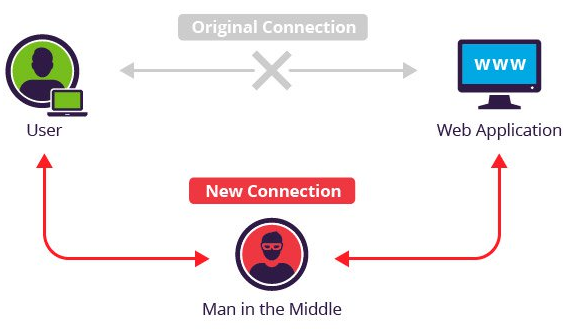
\includegraphics[scale=0.6]{res/img/64_MITM.png}
%\caption{Didascalia dellimmagine}
\end{figure}


\section{DNS spoofing}
\subsection{Cos'è?}
DNS spoofing è una tipologia di attacco crittografico, fa parte di una categoria più vasta denominata man-in-the-middle. Gli attacchi di questo tipo consistono nel deviare i pacchetti di una comunicazione tra due host verso un attaccante. Questo attaccante finge di essere il mittente o il destinatario reale e può leggere, inserire o modificare i dati presenti nella conversazione.

Il protocollo DNS invece ha il compito di trasformare un indirizzo letterale (ad esempio www.fedesimpy.it) in indirizzo numerico o IP (202.159.222.222).
Il DNS Spoofing si svolge quindi nel modo seguente: 
\begin{itemize}
\item	La vittima fa una DNS Query
\item	L’attaccante la intercetta e risponde con una risposta falsa, diversa da quella che sarebbe stata fornita dal DNS.
\end{itemize}
Lo scopo dello spoofing è modificare la corrispondenza tra indirizzo IP e nome del sito contenuti nelle risposte.
\subsection{Possibile soluzione}
Una possibile soluzione per rendersi conto di essere sotto attacco è di individuare possibili risposte multiple. Ci sono altri protocolli utilizzabili per evitare questo tipo di manomissione.

\begin{figure}[H]
\centering
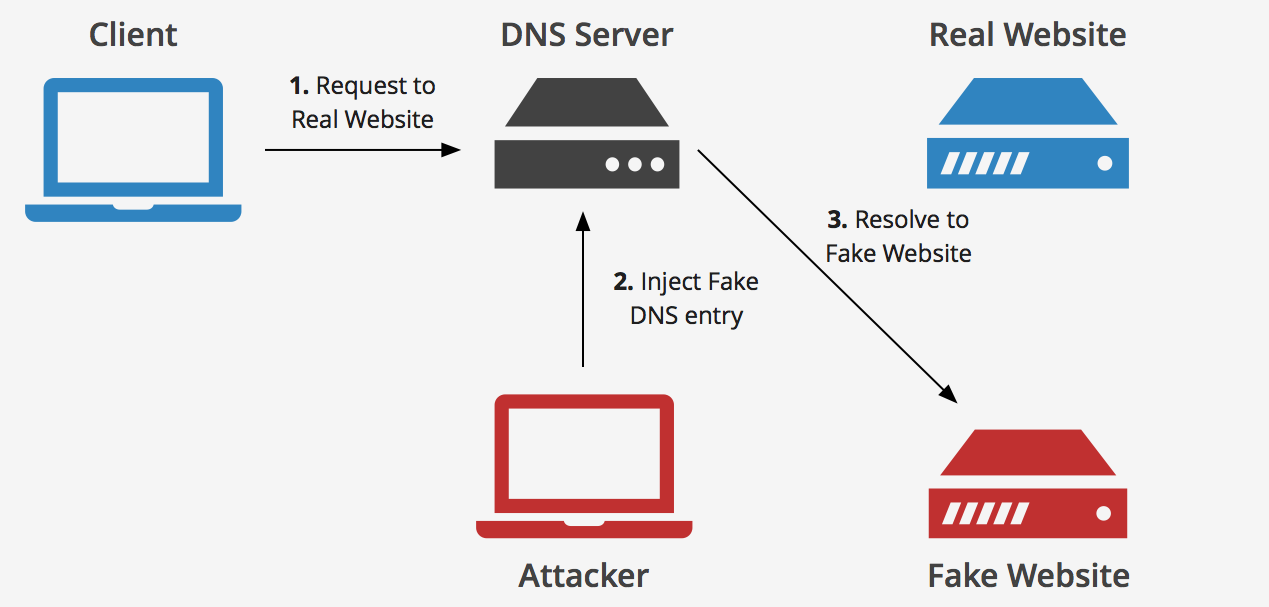
\includegraphics[scale=0.35]{res/img/65_DNSSpoofing.png}
%\caption{Didascalia dellimmagine}
\end{figure}
